%% 
%% Copyright 2019-2020 Elsevier Ltd
%% 
%% This file is part of the 'CAS Bundle'.
%% --------------------------------------
%% 
%% It may be distributed under the conditions of the LaTeX Project Public
%% License, either version 1.2 of this license or (at your option) any
%% later version.  The latest version of this license is in
%%    http://www.latex-project.org/lppl.txt
%% and version 1.2 or later is part of all distributions of LaTeX
%% version 1999/12/01 or later.
%% 
%% The list of all files belonging to the 'CAS Bundle' is
%% given in the file `manifest.txt'.
%% 
%% Template article for cas-dc documentclass for 
%% double column output.

%\documentclass[a4paper,fleqn,longmktitle]{cas-dc}
\documentclass[a4paper,fleqn]{cas-dc}

%\usepackage[authoryear,longnamesfirst]{natbib}
%\usepackage[authoryear]{natbib}
\usepackage[numbers]{natbib}

%%%Author definitions
\def\tsc#1{\csdef{#1}{\textsc{\lowercase{#1}}\xspace}}
\tsc{WGM}
\tsc{QE}
\tsc{EP}
\tsc{PMS}
\tsc{BEC}
\tsc{DE}
%%%
% -------------------------------------------------------------------
% Pacotes para inserção de figuras e subfiguras
\usepackage{subfig,epsfig,tikz,float}		            % Packages de figuras. 
\usepackage{graphicx}
\graphicspath{ {./figs/} }
% -------------------------------------------------------------------
% \usepackage{amssymb}
% -------------------------------------------------------------------
% Pacotes para inserção de tabelas
\usepackage{booktabs,multicol,multirow,tabularx,array}          % Packages para tabela
\usepackage{natbib}
\usepackage{pifont}
\usepackage{xcolor}
% -------------------------------------------------------------------
\PassOptionsToPackage{style=super,nolist}{glossaries}
\PassOptionsToPackage{acronym}{glossaries}
\PassOptionsToPackage{nonumberlist}{glossaries}
\usepackage{glossaries}
\newacronym{ai}{AI}{Artificial Intelligence}
\makeglossaries
% -------------------------------------------------------------------
\usepackage[utf8]{inputenc} % The default since 2018
\DeclareUnicodeCharacter{200B}{{\hskip 0pt}}
% -------------------------------------------------------------------
\begin{document}
\let\WriteBookmarks\relax
\def\floatpagepagefraction{1}
\def\textpagefraction{.001}
\shorttitle{Leveraging social media news}
\shortauthors{CV Radhakrishnan et~al.}


\title [mode = title]{Decentralized File Exchange Hub: A Cloud-Native Approach}                     

\credit{Conceptualization of this study, Methodology, Software}

\author[1]{Rafael Pereira}[type=editor,
                        %auid=000,bioid=1,
                        linkedin='rafaelmendespereira',
                        orcid=0000-0001-8313-7253]
%\cormark[1]
%\fnmark[1]
\ead{rafael.m.pereira@ipleiria.pt}
   
\address[1]{Computer Science and Communications Research Centre, School of Technology and Management, Polytechnic of Leiria, 2411-901 Leiria, Portugal}

\begin{abstract}

In this report, we present a decentralized file exchange hub designed using a cloud-native approach that leverages containers, microservices, and cloud services. Our architecture comprises a React-based frontend served by Nginx, an Express API for managing file transfers, a real-time communication server using Socket.IO, and MongoDB as the primary database. The application stores files in Google Cloud Storage, and our deployment pipeline is streamlined using Google Cloud Build and Cloud Run. The result is a scalable, resilient, and efficient file exchange system that demonstrates the power and flexibility of modern cloud computing technologies for software applications.

\end{abstract}

\begin{keywords}
Decentralized file exchange \sep Microservices architecture \sep Containerization \sep Cloud-native deployment \sep Real-time communication \sep Scalability and resilience
\end{keywords}


\maketitle

\section{Introduction}

The rapid growth of cloud computing and microservices has revolutionized the way applications are developed and deployed. As a result, there is an increasing need for effective strategies to manage the complexity and scalability of these systems. This report explores the design and deployment of a distributed cloud-based application that utilizes containerization and microservices to achieve high availability, performance, and maintainability.

The application is divided into four main modules: Presentation Provider (Nginx), API (Express), Asynchronous Message Communication server, and Database (MongoDB). Each module is designed to serve a specific purpose and can scale independently to adapt to changing loads and requirements. The application also leverages Google Cloud Platform (GCP) services such as Cloud Storage Bucket for storing and managing files.

The report is structured as follows: Section \ref{sec:architecture} presents the architecture of the application, detailing the purpose and design of each module. Section \ref{sec:deployment} describes the deployment process, emphasizing the use of GCP's Cloud Build and Cloud Run services to automate and streamline the deployment of the application components. Finally, the report concludes with a summary of the key findings and insights gained from the project.

\section{Architecture}\label{sec:architecture}

This project follows a microservices architecture, which allows for improved scalability, resilience, and maintainability. The system is divided into four main components, each responsible for a specific aspect of the application. Figure \ref{fig:architecture} presents a diagram of the architecture, illustrating the relationship between each component.

\begin{enumerate}
    \item Presentation Provider (Nginx): This component acts as the frontend server, hosting the React web application and serving static files. It is responsible for delivering the user interface to the clients and handling incoming HTTP requests.
    \item API (Express File Management Service): This component is the backend server implemented using Express.js. It manages the file uploading and downloading processes, interacting with the Database and Cloud Storage Bucket to store and retrieve files.
    \item Asynchronous Message Communication Server (Socket.io): This server enables real-time communication between the clients, ensuring that users in the same room receive instant updates when a new file is shared.
    \item Database (MongoDB): The database stores information about the rooms, users, and file metadata, including the bucket URL and timestamp. MongoDB was chosen for its flexibility, scalability, and performance.
    \item Cloud Storage Bucket (Google Cloud Storage): This component stores the uploaded files, providing a reliable and scalable storage solution.
\end{enumerate}

The following UML diagram (Figure \ref{fig:architecture}) depicts the relationships between the components:

\begin{figure}[h]
    \centering
    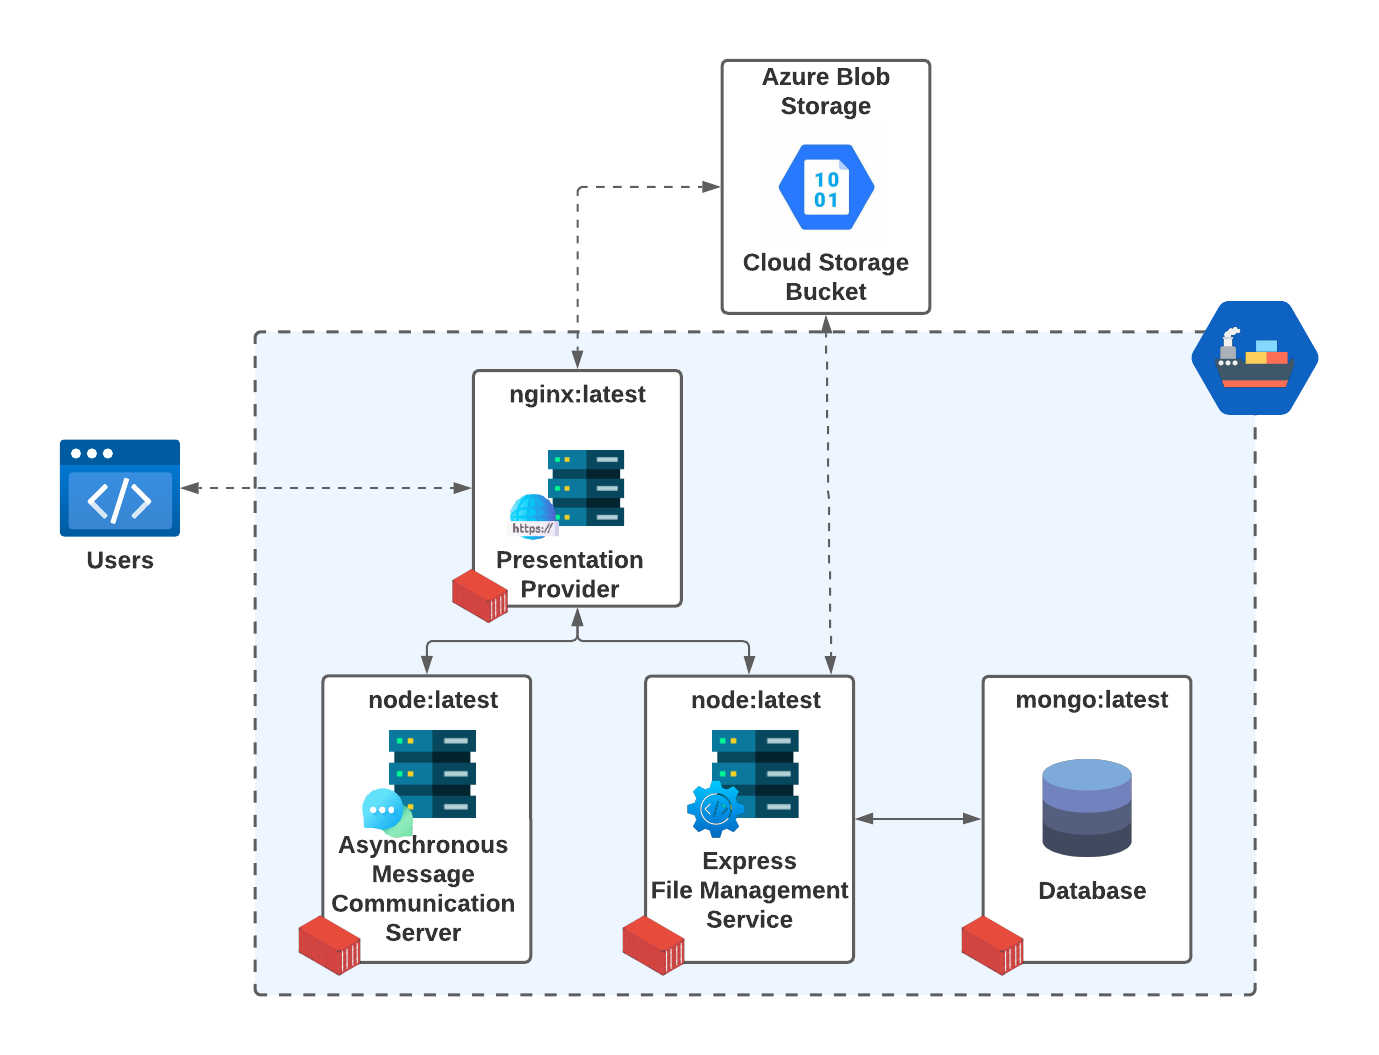
\includegraphics[width=7cm]{architecture.png}
    \caption{System architecture diagram}
    \label{fig:architecture}
\end{figure}

In this architecture, each component communicates with the others through well-defined interfaces, allowing for efficient collaboration and easy maintenance. The use of containerization and cloud-native deployment further enhances the system's scalability and resilience.

\subsection{Presentation Provider: Nginx-based Frontend}

The presentation layer of our file exchange hub is built using a React web application. We utilize Nginx as a reverse proxy and web server to serve the static content generated by the React application. Nginx offers excellent performance, stability, and low resource usage, making it an ideal choice for our frontend.

\subsection{API: Express-based File Transfer Service}

Our file transfer service is implemented using Node.js with the Express framework, providing a robust and scalable API for managing file uploads and downloads. This service is responsible for handling file metadata, coordinating file transfers, and integrating with the cloud storage service for actual file storage.

\subsection{Asynchronous Message Communication Server: Socket.IO}

To enable real-time communication and notifications within our file exchange hub, we employ Socket.IO, a popular library for real-time web applications. This server facilitates instant messaging between users in the same room, ensuring a seamless and interactive experience for all participants.

\subsection{Database: MongoDB}

MongoDB, a NoSQL database, is utilized to store information about rooms, files, and users. It's flexible schema and horizontal scalability makes it a fitting choice for our cloud-native application, as it can easily adapt to changing requirements and handle large volumes of data.

\subsection{Cloud Storage Bucket: Google Cloud Storage}

To store and manage the actual files exchanged by users, we leverage Google Cloud Storage. This fully managed object storage service offers high availability, durability, and scalability, allowing our file exchange hub to efficiently store, retrieve, and share files.

\section{Deployment} \label{sec:deployment}

The deployment process is designed to ensure a smooth transition from development to production, leveraging the power of Google Cloud Platform (GCP) services. The deployment strategy uses GCP's Cloud Build and Cloud Run services for automating and streamlining the process. Figure \ref{fig:deployment} presents a diagram of the deployment process, illustrating the steps and relationships between each involved service.

\begin{enumerate}
    \item Cloud Build: This service automates the build, test, and deployment of the application components. It is triggered when changes are pushed to the repository, and it builds the Docker images for the various services in the application.
    \item Cloud Run: This service deploys the containerized applications on a fully managed platform, providing automatic scaling and load balancing. It ensures that the services are highly available and resilient.
\end{enumerate}

The following UML diagram (Figure \ref{fig:deployment}) depicts the deployment process and the relationships between the components:

\begin{figure}[h]
    \centering
    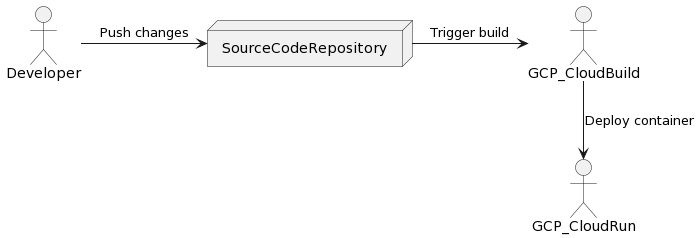
\includegraphics[width=8cm]{deployment.png}
    \caption{Deployment process diagram}
    \label{fig:deployment}
\end{figure}

The deployment process ensures that the application components are consistently built and deployed across environments, minimizing human error and facilitating continuous integration and delivery.


\subsection{Cloud Build: Continuous Integration and Deployment}

For a streamlined development and deployment process, we use Google Cloud Build, a managed service for building, testing, and deploying container images. This service automates the process of building Docker images from our source code and deploying them to Google Cloud Run, ensuring a consistent and reliable deployment pipeline.

\subsection{Cloud Run: Scalable Containerized Services}

Our application's microservices are containerized and deployed on Google Cloud Run, a serverless platform that runs Docker containers. This allows us to easily scale our services up or down based on demand, ensuring optimal resource usage and cost efficiency.

\section{Conclusion}

This report has presented a decentralized file exchange hub designed with a cloud-native approach. By leveraging containers, microservices, and cloud services, we have created a scalable, resilient, and efficient system for exchanging files. Our use of modern technologies such as Nginx, Express, Socket.IO, MongoDB, and Google Cloud services demonstrates the power and flexibility of cloud computing for modern software applications.

%% Loading bibliography style file
%\bibliographystyle{model1-num-names}
%\bibliographystyle{cas-model2-names}
\bibliographystyle{unsrt} % Estilo de Bibliografia
% Loading bibliography database
\bibliography{cas-refs}


%\vskip3pt

\bio{figs/bioFig}
My name is Rafael Pereira, I'm 22 years old, and I'm an MSc Computer Engineering Student and Researcher at Polytechnic of Leiria. I'm extremely curious about the technology world, ambitious for knowledge in this area, I'm dedicated to doing my work. The programming thing always got me, and every day it grows. Today I'm looking for interesting projects, that can make me think and learn every day.
\endbio

\end{document}
